\chapter{JSP(Java Server Page)}
\label{chp:JavaEE-HTTP-session}

\section*{基本信息}
\sline
\begin{description}
\item[课程名称:] Java应用与开发
\item[授课教师:] 王晓东
\item[授课时间:] 第十三周
\item[参考教材:] 本课程参考教材及资料如下:
  \begin{itemize}
  \item 吕海东,张坤 编著,Java EE企业级应用开发实例教程,清华大学出版社,2010年8月
  \end{itemize}
\end{description}

\section*{教学目标}

\sline

\begin{enumerate}
\item 理解JSP和Servlet的关系。
\item 掌握JSP提供的各类编程元素的使用方式,包括JSP指令、JSP动作、JSP脚本。
\item 掌握JSP提供的内置对象与Servlet相关对象的对应,学会各类对象的使用方法。
\item 能够使用JSP完成简单的Java Web编程。
\item 对JSP作为MVC设计模式中的视图构建方式有初步的了解。  
\end{enumerate}  


\section*{授课方式}

\sline
\begin{description}
\item[理论课:] 多媒体教学、程序演示
\item[实验课:] 上机编程
\end{description}

\newpage
\section*{教学内容}
\sline

%%%%%%%%%%%%%%%%%%%%%%%%%%%%%%%%%%%%%%%%%%%%%%%%%%%%%%%%%%%%%%
\section{JSP概述}

\subsection{JSP基本概念}

\begin{itemize}
\item JSP(Java Server Page),即Java服务器页面。
\item JSP是Servlet的扩展。
\item {\bf\Blue JSP将使用Java类编写动态Web组件的方式转变为使用文本编
    写(采用标记型语法和过程性语法混合),降低了开发的难度。}
\item JSP提供了一种自然的生成网页的方法。
\item 可以使用GUI工具来绘制构建JSP页面。
\item JSP文件的扩展名必须是 .jsp。
\end{itemize}

\subsection{JSP的优点和缺点}

\tta{优点}

\begin{itemize}
\item 使得编写动态Web网页更加容易;
\item 降低了开发难度;
\item 可以使用工具的拖拉方式生成JSP页面。
\end{itemize}

\tta{缺点}

\begin{itemize}
\item 非OO编程方式;
\item Java代码嵌入到HTML代码中,导致维护困难;
\item 不适合编写规模比较大的业务处理应用程序。
\end{itemize}


\subsection{JSP的执行过程} 

\begin{figure}[htb]
\centering
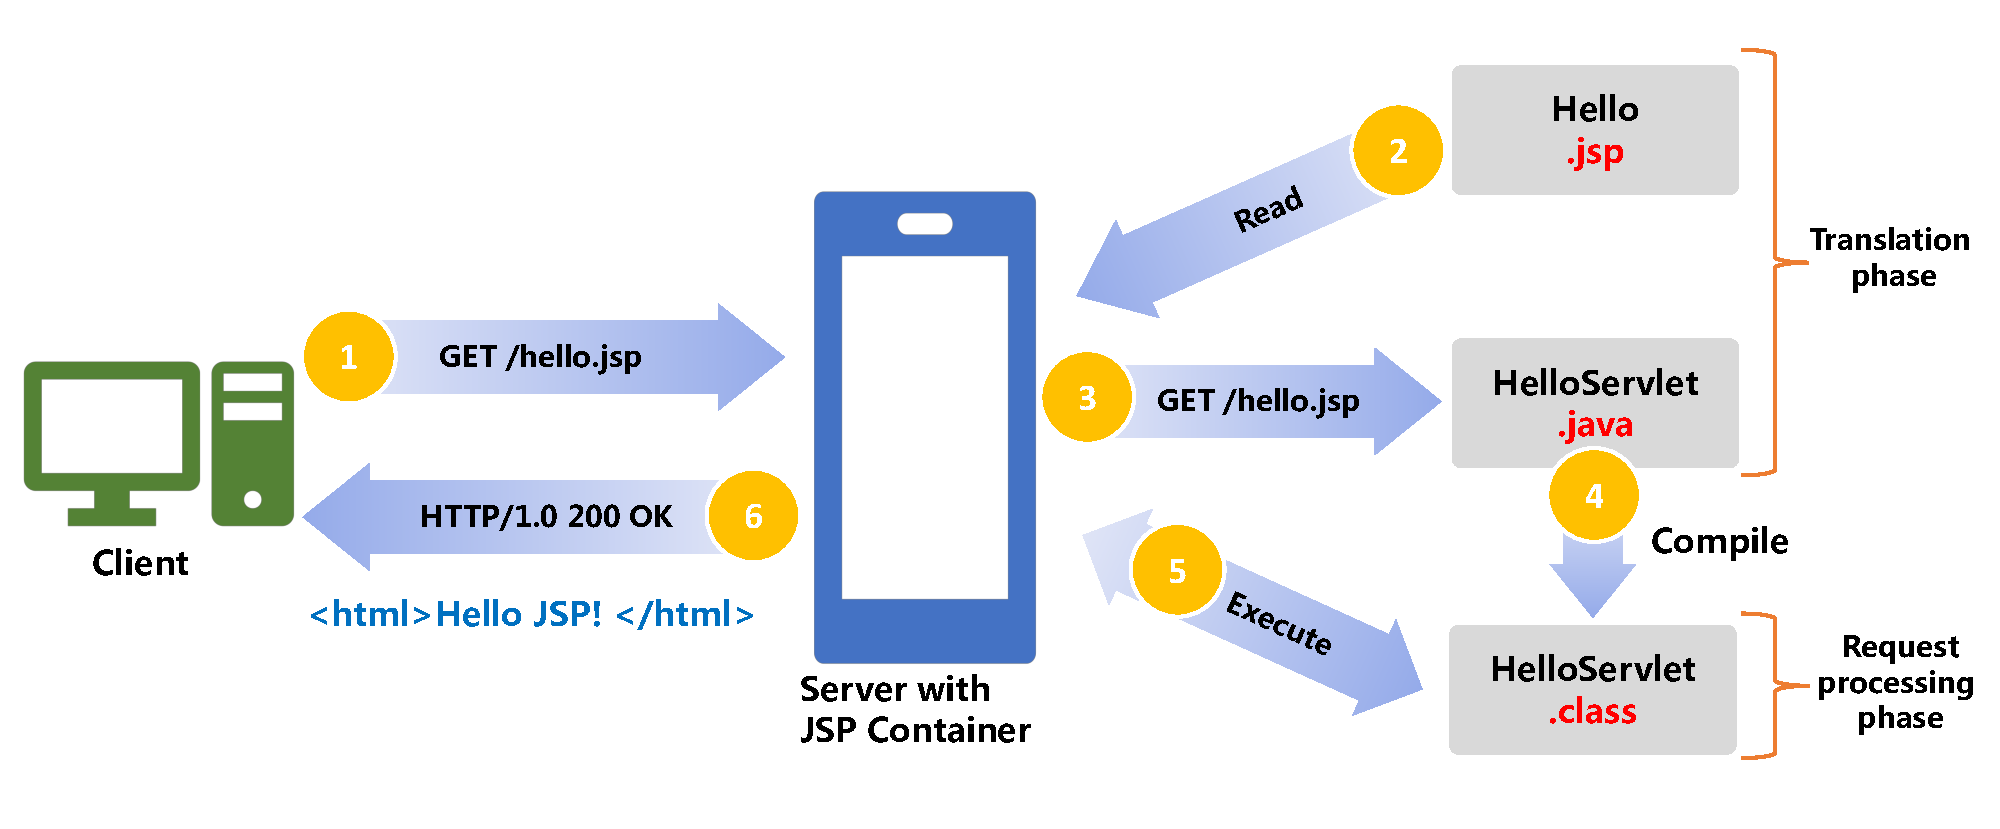
\includegraphics[width=0.8\textwidth]{images/JavaEE-JSP/fig-jsp-process.pdf}
\caption{JSP的执行过程}
\label{fig:fig-jsp-process}
\end{figure}

\subsection{JSP执行过程描述} 

\begin{enumerate}\kai
\item 客户使用浏览器通过HTTP请求JSP文件的URL地址,
  例如:http://localhost:8080/webapp/hello.jsp;
\item Web服务器接收到请求,如果没有此地址,发出错误响应给浏览器;
\item Web服务器检查JSP文件和对应的Servlet版本的时间是否一致,如果一致则
  执行servlet的处理请求方法,类似于doGet或doPost,发送响应给浏览器;
\item 版本时间不一致,Web服务器调用转换系统,将JSP的文本代码转换为Servlet的Java代码;
\item 将Java代码编译为class文件;
\item 调用Servlet Class的相应方法处理请求并返回响应。
\end{enumerate}

\subsection{JSP页面的组成} 

一个JSP页面由{\hei HTML标记代码}和{\hei JSP元素}组成。HTML标记用于生
成网页的静态部分,JSP元素用于生成动态内容部分。

JSP所包含的元素主要包括JSP指令、JSP动作、JSP脚本、JSP内置对象和JSP扩展标记。

\section{JSP指令}

JSP指令指示一个JSP页面的属性和特征,JSP指令不会产生任何的输出到当前输出流中。

\tta{JSP指令}
\begin{itemize}
\item page指令,用于定义JSP页面级的其他元素特征。
\item include指令,用于嵌入另一个文本文件的内容到本页面。
\item taglib指令,用于引入第三方JSP扩展标记类库。
\end{itemize}

\tta{JSP指令的语法}

\begin{jspCode}
  <%@ 指令名 属性名="值" 属性名="值" %>  
\end{jspCode}
  
\subsection{page指令}
page指令定义应用于整个页面的属性。

\tta{page指令语法}

\begin{jspCode}
  <%@ page 属性名="属性值"  %>  
\end{jspCode}

\tta{page指令属性}

\begin{itemize}
\item language="java",指定页面语言。
\item contentType="text/html; charset=gb2312",指定页面的内容类型,默认是text/html,可以指定显示的字符集,中文是gb2312 。
\item import="package, pageage",指定JSP页面使用的包和类,可以引用多个包,每个包用逗号分隔。
\item buffer="none | xkb",指定输出缓冲区容量,默认为8KB,buffer="9kb"。
\item errorPage="errorURL",指定错误页面地址,当页面出现异常时自动跳转到指定的错误页面。
\item isErrorPage="true|false",指定本页面是否是错误处理页面。
\item autoFlush="true | false",控制输出缓冲区是否自动清空,默认是true。
\end{itemize}

\subsection{include指令}

include指令用于在当前网页中嵌入另一个网页,可以是JSP、HTML等。

\tta{include指令语法}

\begin{jspCode}
  <%@ include file="url" %>
\end{jspCode}

\notice{说明}

\begin{itemize}
\item file属性确定要嵌入的页面。
\item 嵌入页面的源代码被放置在此指令所在的位置。
\item 嵌入的用途是将一个复杂的页面分解为小的页面,然后使用include指令将他们再组装在一起。
\item {\Red 当修改被include的文件时,如果不修改主文件,则嵌入的内容不会改变。因此必须也修改主文件才能反映更新的嵌入文件。}
\end{itemize}

\subsection{taglib指令} 

taglib指令用于引入扩展标签库,如JSTL、Struts等标签库。

\tta{taglib指令语法}

\begin{jspCode}
  <%@ taglib uri="/WEB-INF/tlds/struts-html.tld" prefix="html" %> 
  <%@ taglib uri="http://java.sun.com/jsp/jstl/core" prefix="c" %>  
\end{jspCode}

\section{JSP动作}

JSP动作使用特定的符合XML格式的标记完成特定的任务。利用JSP动作可以完成动
态的插入文件、重用JavaBean组件、把用户重定向到另外的页面、为Java插件生
成HTML代码。

\tta{JSP动作的语法}

\ttc{无嵌套封闭格式}

\begin{jspCode}
  <jsp:动作名称 属性名="值" 属性名="值" 属性名="值"/>
\end{jspCode}

\ttc{有嵌套封闭格式}

\begin{jspCode}
  <jsp:动作名称 属性名="值" 属性名="值" 属性名="值">
    嵌入的其他动作
  </jsp:动作名称>
\end{jspCode}

\subsection{JSP动作的类型} 

\begin{description}
\item[<jsp:include>] 嵌入其他页面输出内容动作
\item[<jsp:forward>] 转发动作
\item[<jsp:plugin>] 引入插件动作
\item[<jsp:param>] 提供参数动作
\item[<jsp:useBean>] 使用JavaBean动作
\item[<jsp:setProperty>] 设置JavaBean属性动作
\item[<jsp:getProperty>] 取得JavaBean属性动作
\end{description}

\subsection{include动作} 

include动作用于嵌入其他页面的输出内容到此动作所在页面。


\begin{jspCode}
  <jsp:include page="url" flush="true" />
\end{jspCode}

\begin{jspCode}
  <jsp:include page="url" flush="true">
    <jsp:param name="参数名" value="参数值" />
  </jsp:include>
\end{jspCode}

\begin{itemize}
\item page属性,指定嵌入页面的URL地址;
\item flush属性,指定是否在嵌入页面之前清空响应缓存区,默认为true;
\item jsp:param,为嵌入的页面传递参数,这些参数可以为动态、也可以为静态。
\end{itemize}

之前我们讲过include指令,include指令和include动作的差异包括:

\begin{itemize}
\item 其根本性不同在于他们被调用的时间。include指令在页面解析期间被嵌入;inlcude动作在请求的响应输出时被嵌入。
\item {\hei\Red 在实现文件包含上,因该尽可能的使用include动作。}
\item 而include指令存在的原因是其功能更加强大,执行速度稍快。
\end{itemize}

\begin{figure}[htb]
\centering
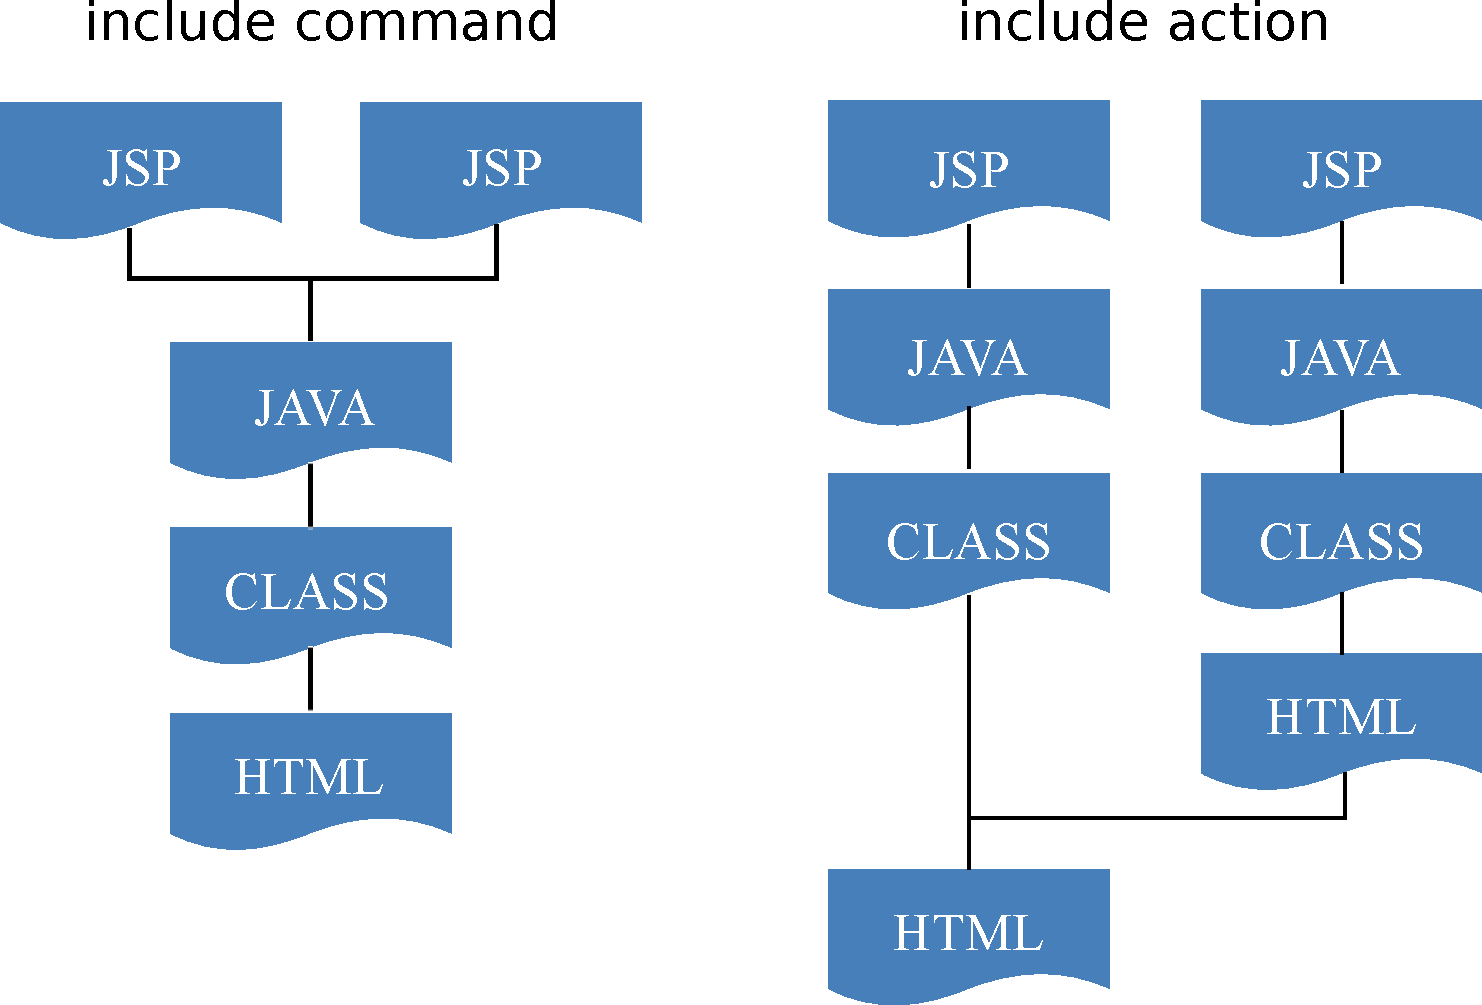
\includegraphics[width=0.6\textwidth]{images/JavaEE-JSP/fig-include-action-and-command.pdf}
\caption{inlcude动作和指令的差异}
\label{fig:include-action-and-command}
\end{figure}

\subsection{useBean动作} 
\begin{itemize}
\item 引用并调用JavaBean的方法和属性是JSP开发时必须面对的主要任务。
\item 为了简化JavaBean应用,JSP提供了useBean动作标记,使得不必使
  用Java脚本代码,而使用标记方式就可以取得JavaBean的对象引用。
\end{itemize}
  
\subsubsection{useBean动作语法}

\begin{jspCode}
  <jsp:useBean id="name" class="package.ClassName" 
    scope="page|request|session|application" />
\end{jspCode}

\begin{itemize}
\item id="name" 实例化变量名
\item scope="scope" 定义实例变量的生存周期范围
  \begin{itemize}\kai\small
  \item page只在本页面中使用,默认值
  \item request在请求范围内有效
  \item session在会话范围内有效
  \item application在整个Web启动后有效
  \end{itemize}
\item class="package.ClassName" 指定JavaBean的类
\end{itemize}

\subsubsection{useBean的执行过程}

\begin{enumerate}\kai
\item 如果在指定范围内找到指定的对象,则得到此对象引用(即通过scope对象的getAttribute()方法)。
\item 如果没有找到指定的对象,则实例化一个class属性指定的对象(调用类的无参数构造方法)。
\item 对新建的对象执行嵌入的<jsp:setProperty />中指定的属性值,即调用JavaBean的setXXX方法,设置类的属性值。
\item 将对象保存到scope指定的范围的对象中,即调用内置对象的setAttribute(name,Object)方法,name是id指定的名称,object是类的对象。
\end{enumerate}

\subsubsection{useBean动作示例} 

\ttc{JavaBean类User:User.java}

\begin{javaCode}
  package ouc.java.entity;
  import java.io.Serializable;  
  public class User implements Serializable {
    private String id = null;
    private String password = null;
    private String name = null;
    private age = 0;

    public String getId() {
      return id;
    }
    public void setId(String id) {
      this.id = id;
    }
    ... ... // (other set/get methods.)
  }
\end{javaCode}

\ttc{创建/取得指定的JavaBean对象,并保存在Request对象中}

\begin{jspCode}
  <jsp:useBean id="user" class="ouc.java.entity.User" scope="request" \>
  <%
    String name = user.getName();
    out.println(name);
  %>
\end{jspCode}

\subsubsection{使用useBean动作 VS. JSP脚本创建并取得对象引用} 

\tta{使用JSP脚本}

\begin{jspCode}
  <% User user = new User(); %>
\end{jspCode}

\notice{注意}

以上使用Java脚本创建的JavaBean,只能在本页面中使用,且每次都是创建新
的JavaBean对象,不会保存在任何范围对象中。

\tta{使用JSP动作}

\begin{jspCode}
  <jsp:useBean id="user" class="ouc.java.entity.User" scope="request" \>
\end{jspCode}

以上使用JSP动作代码,相当于如下Java脚本:

\begin{jspCode}
  <%
    User user = (User) request.getAttribute("user");
    if (user == null) {
      user = New User();
      request.setAttribute("user", user);
    }
  %>
\end{jspCode}

\subsection{setProperty动作} 

setProperty动作用于设定userBean动作取得的Bean对象的属性,相当于执行Bean对象的setXxx方法。

\begin{jspCode}
  <jsp:setProperty name="beanId" property="*|name" param="参数名" value="value" />
\end{jspCode}

\begin{jspCode}
  <jsp:useBean id="user" class="com.city.oa.value.User" scope="request" />
  <jsp:setProperty name="user" property="name" value="吴明" >
\end{jspCode}

\subsection{getProperty动作} 

用于取得Bean对象指定的属性值,转换为String类型,并显示在此动作所在的位置。

\begin{jspCode}
  <jsp:getProperty name="beanId" property="属性名" />
\end{jspCode}

\begin{itemize}
\item name指定bean对象的名称,与useBean动作的id值对应;
\item property指定属性名,与JavaBean的getXxx方法对应。
\end{itemize}

\subsection{forward动作} 

forward动作把请求转到另外的页面。

\ttc{无嵌入参数的转发动作}
\begin{jspCode}
  <jsp:forward page="URL" />
\end{jspCode}

例如:
\begin{jspCode}
  <jsp:forward page="main.jsp" />  
\end{jspCode}

\ttc{有嵌入参数的转发动作}

\begin{jspCode}
  <jsp:forward page="URL">
    <jsp:param name="参数名" value="值" />
  </jsp:forward>
\end{jspCode}

例如:
\begin{jspCode}
  <jsp:forward page="main.jsp">
    <jsp:param name="id" value="kevin" />
    <jsp:param name="password" value="1000" />
  </jsp:forward>
\end{jspCode}

\subsection{param动作} 

param动作不能单独使用,需要嵌套在其他动作中,为其他动作提供参数,它可
以嵌入到include、forward动作中为目标地址提供参数。

\begin{jspCode}
  <jsp:forward page="main.jsp">
    <jsp:param name="id" value="kevin" />
    <jsp:param name="password" value="1000" />
  </jsp:forward>
\end{jspCode}

\section{JSP脚本}

\subsection{代码脚本}
  
\begin{jspCode}
  <%
    int a=0; // 可以放置任何 Java 代码
  % >
\end{jspCode}  
\begin{itemize}
\item 可以同时嵌入多个脚本代码段,但它们都表示在一个方法内,属于一个代码段,一个脚本内定义的变量,另一个脚本也可以使用。
\item 在代码脚本中定义的变量类似于Servlet的doGet方法中的局部变量,未初始化使用是非法的。
\end{itemize}

{\kai 例如,连接数据库的代码脚本片段如下:}
\begin{jspCode}
  <%
  Connection cn = null;
  try {
    Class.forName("sun.jdbc.odbc.JdbcOdbc.Driver");
    cn  = DriverManager.getConnection("jdbc:odbc:cityoa");
    String sql = "select * from EMP";
    ... ...
  }
  % >
\end{jspCode}

\subsection{表达式脚本}

\begin{jspCode}
  <%= a %> 用于输出 Java 表达式的值
\end{jspCode}

\notice{注意}

表达式后不能有分号,=号与<\%之间不能有空格。例如:

\begin{jspCode}
  <%= rs.getString("NAME") %>
\end{jspCode}


\subsection{声明脚本}

\begin{jspCode}
  <%!
    int m=0; // 声明 JSP 类变量和方法
  % >
\end{jspCode}

用于声明JSP页面的类变量和方法。

由于JSP在运行时会转换为Servlet类,声明的脚本部分会成为类中定义的一部分。
例如:

\begin{jspCode}
<%!
  int num = 0;
  public void addNum() {
    num++;
  }
%>
\end{jspCode}

如下声明脚本有错误:

\begin{jspCode}
<%!
  int num = 0;
  num++; // 错误,声明脚本中不能直接有非声明代码
%>  
\end{jspCode}

\subsection{注释脚本}

\begin{jspCode}
  <%-- JSP Comment --%>  
\end{jspCode}

在JSP页面中可以使用HTML注释:

\begin{jspCode}
  <!-- HTML Comment -->
\end{jspCode}

{\kai\Red 但是,使用HTML注释不安全,因为HTML注释随着JSP生成的HTML响应下载到客户端浏览器,客户可以看到。}

JSP注释是服务器端技术,在服务器端处理,不会发送到客户端,比较安全。


\section{JSP内置对象} 


为了与Web容器以及其他Web组件进行通信和协作,JSP提供了相关内置的对象,这
些对象不需要定义和引用,可以在JSP代码脚本和表达式脚本中可以直接使用。

\begin{description}
\item[request] 请求对象
\item[response] 响应对象
\item[session] 会话对象
\item[application] 应用服务器对象
\item[page] JSP本身页面类对象
\item[pageContext] 页面级环境变量,作为页面级容器
\item[out] 输出对象
\item[exception] 异常对象
\item[config] 配置对象,用于读取web.xml配置信息
\end{description}

%%%%%\begin{frame}[fragile] % [fragile]参数使得能够插入代码
%%%%%\subsection{请求对象request} 
%%%%%request与Servlet中传递的请求对象相同,类型为javax.servlet.http.HttpServletRequest。
%%%%%\ttc{常见方法}
%%%%%\begin{itemize}
%%%%%\item Object getAttribute(String name) 返回指定属性的属性值
%%%%%\item Enumeration getAttrbuteNames() 返回所有可用属性名的枚举
%%%%%\item String getCharacterEncoding() 返回字符编码的方式
%%%%%\item String getParameter(String name) 返回指定参数的参数值
%%%%%\item ...
%%%%%\end{itemize}
%%%%%\end{frame}
%
\subsection{响应对象response} 

\begin{itemize}
\item JSP页面使用文本方式实现HTTP响应,所以JSP内部不经常使
  用response对象。
\item 在JSP中实现响应,直接将响应内容写在JSP页面就可以,不需要使用响
  应对象取得PrintWriter对象进行响应输出。
\end{itemize}

\subsection{会话对象session} 

\begin{itemize}
\item JSP的session对象对应Servlet中的{\bf\Blue javax.servlet.http.HttpSession}。
\item JSP页面使用page指令指示此JSP页面是否可以使用session内置对象。
\end{itemize}

\begin{jspCode}
  <%@ page session="true | false" %> 
\end{jspCode}

%%%%%\ttc{常见方法}
%%%%%\begin{itemize}\kai\small
%%%%%\item long getCreationTime() 返回session创建时间
%%%%%\item public String getId() 返回session创建是JSP引擎为它设置的唯一ID号
%%%%%\item long getLastAccessdTime() 返回此session中客户端最近一次请求的时间
%%%%%\item int getMaxInactiveInterval() 返回两起请求间隔多长时间此session被取消
%%%%%\item String[] getValueNames() 返回一个包含此session中所有可用属性的数组
%%%%%\item void invalidate() 取消session,使其不可用
%%%%%\end{itemize}
%\end{frame}
%
%%%%%\begin{frame}[fragile] % [fragile]参数使得能够插入代码
%%%%%\subsection{服务器环境对象application} 
%%%%%\begin{itemize}
%%%%%\item appliation对应Servlet中的javax.servlet.ServletContext对象实例。
%%%%%\item 每个Web站点只有一个application对象。
%%%%%\item application对象是一个Map类型的容器。
%%%%%\item application作为Web级的容器,保存整个Web应用个Web组件之间需要共享的数据,application可以保存整个请求用户都可以访问的共享信息。
%%%%%\item 在保存信息到application时,要注意多用户同时写的线程同步问题。
%%%%%\end{itemize}
%%%%%
%%%%%\ttc{常用方法}
%%%%%\begin{itemize}
%%%%%\item 存入数据方法 void setAttribute(String name,Object object);
%%%%%\item 读取数据的方法 Object getAttribute(String name);
%%%%%\item 删除数据的方法 void removeAttribute(String name);
%%%%%\end{itemize}
%%%%%\end{frame}
%

\subsection{页面对象page} 

page对象就是指向当前JSP页面本身,有点像类中的this指针,它是java.lang.Object的实例,在JSP编程中应用较少。

\ttc{常用方法}

\begin{itemize}
\item int hashCode() 返回此Object的hash码
\end{itemize}

%%%%%\begin{frame}[fragile] % [fragile]参数使得能够插入代码
%%%%%\subsection{页面环境对象pageContext} 
%%%%%略。
%%%%%\end{frame}

\subsection{输出对象out}

out内置对象即JSP页面向浏览器发出响应流PrintWriter的实例对象。但JSP页面
可以直接放入响应文本,因此JSP页面基本不使用out进行文本响应。

一般情况下使用{\bf\Red JSP表达式脚本}来代替使用out对象。

\begin{jspCode}
  <%= %>  
\end{jspCode}

\subsection{异常对象exception} 

JSP内置对象exception对应Java中的java.lang.Throwable接口对象。它自动封
装JSP页面中出现的异常。

异常对象只有在{\hei\Blue 错误页面}中可以使用,即:{\kai\Red 使用page指令的属
  性{\Blue isErrorPage="true"}声明的页面。}

\ttc{sample.jsp}

\begin{jspCode}
  <%@ page language="java" contentType="text/html; charset=utf-8" 
    errorPage="error.jsp" import="java.util.*" pageEncoding="utf-8" %>
  <html>
    <head>
      <meta http-equiv="Content-Type" content="text/html; charset=utf-8">
      <title>Test Exception</title>
    </head>
    <body>
      <%
        int s = 0;
        int t = 0; 
        int p = s / t; // 出现异常的语句
      %>
    </body>
  </html>  
\end{jspCode}

\ttc{error.jsp}

\begin{jspCode}
  <%@ page language="java" contentType="text/html; charset=utf-8" isErrorPage="true"
    pageEncoding="utf-8"%>
  <html>
    <head>
      <meta http-equiv="Content-Type" content="text/html; charset=utf-8">
      <title>Error Page</title>
    </head>
    <body>
      <h1>异常显示信息</h1>
      错误原因:<%= exception.getMessage() %>
    </body>
  </html>  
\end{jspCode}

{\kai\Red 使用errorPage方式实现的页面跳转,使用的是转发方式,而不是重定向模式。}


%%%%%\begin{frame}[fragile] % [fragile]参数使得能够插入代码
%%%%%\subsection{配置对象config} 
%%%%%
%%%%%congfig对象提供对JSP页面的javax.servlet.ServletConfig对象的访问。例如:
%%%%%
%%%%%\begin{jspCode}
%%%%%<%= config.getInitParameter("driverName") %>
%%%%%\end{jspCode}
%%%%%\end{frame}


\section{课后习题}

\tta{简答题}

\begin{enumerate}
\item 什么是JSP?JSP运行在哪里?JSP一般的输出是什么?
\item JSP有哪些优点和缺点?
\item JSP的执行过程是怎样的?
\item 能够基于一个简单的JSP页面代码进行分析,找出JSP转换为Servlet后,相
  关JSP元素在Servlet中都是如何转换的。
\end{enumerate}

\tta{小编程}

\begin{enumerate}
\item 整理一份你最喜欢的歌单,最少包括10首歌曲,并将歌单存入MySQL数据库。每首歌曲需要包括曲名、演唱者、类型风格等信息。
\item 编写JSP代码,直接在JSP中连接数据库并查询歌单,将所有歌曲信息以HTML table的形式显示在页面上。
\item 注意可能会用到JSTL标记实现table的循环生成行,请自行检索简单用法。
\end{enumerate}
